% P0 - VTS 2027 regular paper draft
% Build: pdflatex main && pdflatex main
\documentclass[conference]{IEEEtran}
\usepackage{graphicx}
\usepackage{booktabs}
\usepackage{amsmath}
\usepackage{cite}
\usepackage{xcolor}
\usepackage{tikz}
\usetikzlibrary{positioning,arrows.meta,fit}
\usepackage[hidelinks]{hyperref}
\graphicspath{{../figs/}{../results/waves/}}

\begin{document}

\title{Beyond Pass/Fail: Golden-Model Verification\\of MBIST and Self-Repair Logic}

\author{\IEEEauthorblockN{Abhinav Kidambi, IEEE Member}
\IEEEauthorblockA{Independent Researcher, USA\\
abhinavkidambi1989@gmail.com}}

\maketitle

\begin{abstract}
Memory built-in self-test (MBIST) and built-in self-repair (BISR) logic decide whether a
defective memory is shipped, repaired or discarded, yet their RTL is commonly verified only by
checking that the test completes and that its pass/fail flag looks plausible. We present a
golden-model verification method that checks every observable MBIST/BISR result (the pass/fail
flag, each reported fail address and the final repair table) against an operation-level March
reference model under systematic memory fault injection, and qualifies the checker itself with
seeded RTL bugs. On an open-source MBIST/BISR design taped out on a public shuttle, 4{,}032
injected stuck-at, transition and coupling faults show that its completion-only testbench
exposes no bug and a pass/fail check exposes only 2.8\% of detectable faults (72 escapes,
95\% CI 2.3--3.6\%), whereas the full scoreboard exposes bugs in 100\% of them: every fail
address and repair entry is wrong and the faulty cell is repaired in only 1.6\% of failing runs.
On a second open-source MBIST with row-redundancy repair the same scoreboard raises no false
alarm in 1{,}694 runs (95\% upper bound 0.23\%). Across 34 seeded bugs, completion-only checking
kills 15\%, pass/fail checking 62\% and the full scoreboard 79\%. The flow uses only open-source
tools and runs in seconds to minutes.
\end{abstract}

\begin{IEEEkeywords}
MBIST, built-in self-repair, March test, memory fault models, fault injection, mutation analysis, design verification
\end{IEEEkeywords}

\section{Introduction}
Embedded memories dominate the area of modern SoCs, and nearly every memory instance is wrapped
in MBIST and, increasingly, repair logic \cite{zorian2003}. A bug in this logic is costly in both
directions: a missed fault ships a defective part, while a wrong fail address or repair entry
wastes redundancy or ``repairs'' a good cell and leaves the bad one in use. Because MBIST runs
on every die at every insertion, such a bug is replicated across the whole product.

In practice MBIST RTL is often verified by running the test on a fault-free memory and checking
that DONE rises and FAIL stays low, sometimes with a few injected faults checked for FAIL. Such
checks say little about the information that repair and diagnosis consume: \emph{which}
addresses failed, and \emph{what} was written into the repair registers. They also say nothing
about how many real bugs the checks themselves would miss.

This paper contributes (a) a reference-model-driven method that predicts, for any injected fault,
the pass/fail flag, the ordered fail-address list and the repair table, and scores the RTL at
three increasing checker levels (Section~\ref{sec:method}); (b) an open-source fault-injection and
seeded-bug campaign flow with confidence intervals for every rate (Section~\ref{sec:setup}); (c) a
case study on a taped-out MBIST/BISR design in which the method finds escapes, wrong fail
addresses and a broken repair table that the design's own testbench misses, with register-level
root causes (Sections~\ref{sec:resA}--\ref{sec:root}); (d) a control study on a second design in
which the same scoreboard raises no false alarm, and a seeded-bug qualification of all checker
levels on both designs (Sections~\ref{sec:resB}--\ref{sec:mut}); and (e) design recommendations
for MBIST/BISR logic (Section~\ref{sec:disc}).

\section{Background and Related Work}
\label{sec:background}
\textbf{March tests.} A March test applies March elements, each a series of reads and writes
applied to every address in ascending ($\Uparrow$), descending ($\Downarrow$) or either
($\Updownarrow$) order \cite{vandegoor1991,vandegoor1993}. MATS+ \cite{knaizuk1977,vandegoor1991}
detects stuck-at faults (SAF) in $5N$ operations; March X ($6N$) and March Y ($8N$) add
transition faults (TF); March C-- \cite{marinescu1982,vandegoor1993},
$\{\Updownarrow(w0);\Uparrow(r0,w1);\Uparrow(r1,w0);\Downarrow(r0,w1);\Downarrow(r1,w0);\Updownarrow(r0)\}$,
detects all SAFs, TFs, address-decoder faults and unlinked inter-word idempotent coupling faults
(CF) in $10N$. Intra-word CFs need several data backgrounds \cite{vandegoor1991}; linked faults
need longer tests \cite{vandegoor1996,alharbi2003}.

\textbf{Verifying memory tests and MBIST.} Van de Goor and Smit automated the verification of
March \emph{algorithms} against fault models \cite{vandegoor1994}; that work does not check the RTL
that implements an algorithm. Assertion-based verification has been applied to March-based MBIST
controllers \cite{kumar2021}, and a recent industrial methodology closes coverage gaps in
shared-bus MBIST with physical-design-aware checks \cite{tulsyan2026}.

\textbf{Repair and testbench quality.} BISR stores failing addresses and remaps accesses to spare
rows, columns or words \cite{zorian2003,sontakke2024}, so its correctness depends directly on the
fail addresses MBIST reports. Mutation analysis \cite{demillo1978,jia2011} measures how many
seeded bugs a test environment detects.

We differ from these works in checking, against a golden model, \emph{every} result an MBIST/BISR
block produces under a systematic fault campaign, in quantifying what weaker checkers miss with
both injected faults and seeded RTL bugs, and in being reproducible with open designs and tools.

\section{Method}
\label{sec:method}
Fig.~\ref{fig:method} shows the flow. For each fault, the testbench injects it into the
behavioural memory of the unmodified RTL, runs MBIST to completion and records every fail report
and the final repair table. Independently, the golden model applies the specified algorithm to
an operation-level memory with the same fault and predicts the correct results. A scoreboard
compares the two at three checker levels and writes one row per run.

\begin{figure}[t]
\centering
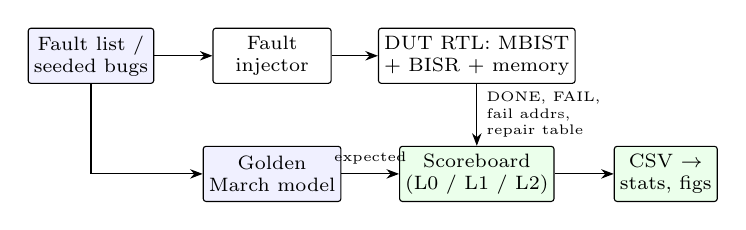
\begin{tikzpicture}[font=\scriptsize,
  box/.style={draw, rounded corners=1pt, align=center, minimum height=7mm, minimum width=15mm, inner sep=2pt},
  >={Stealth[length=1.6mm]}]
\node[box, fill=blue!6] (fl) at (0,0) {Fault list /\\seeded bugs};
\node[box] (inj) at (2.3,0) {Fault\\injector};
\node[box, minimum width=19mm] (dut) at (4.9,0) {DUT RTL: MBIST\\+ BISR + memory};
\node[box, fill=blue!6] (gm) at (2.3,-1.5) {Golden\\March model};
\node[box, minimum width=19mm, fill=green!8] (sb) at (4.9,-1.5) {Scoreboard\\(L0 / L1 / L2)};
\node[box, minimum width=12mm, fill=green!8] (csv) at (7.3,-1.5) {CSV $\rightarrow$\\stats, figs};
\draw[->] (fl) -- (inj);
\draw[->] (inj) -- (dut);
\draw[->] (fl) |- (gm);
\draw[->] (dut) -- node[right, align=left, font=\tiny] {DONE, FAIL,\\fail addrs,\\repair table} (sb);
\draw[->] (gm) -- node[above, font=\tiny] {expected} (sb);
\draw[->] (sb) -- (csv);
\end{tikzpicture}
\caption{Verification flow. Blue: inputs and golden reference; white: unmodified RTL with behavioural fault injection; green: scoring and statistics.}
\label{fig:method}
\end{figure}

\subsection{Golden model}
The golden model simulates a $D\times W$ memory at the operation level. An algorithm is a list of
(order, operations) pairs, optionally repeated for a list of data backgrounds, with data `0' the
background and `1' its complement. Each read compares the whole word; a mismatching read appends
its address to the expected fail list. The expected repair table is the first $R$ distinct failing
addresses in detection order. Spare words are assumed fault-free and outside the tested range,
the documented intent of both designs. The model reproduces March theory on our fault list
(Fig.~\ref{fig:alg}): MATS+ detects 50\% of TFs, March X and March Y 50\% of inter-word CFs,
March C-- all of them, and four data backgrounds all intra-word CFs.

\subsection{Fault injection}
Faults are injected into the RTL memory array without editing the design. A correction is applied
just after every clock edge, after any write has landed and before the next read samples the
array: an SAF forces the cell; a TF reverts a forbidden $0\!\to\!1$ or $1\!\to\!0$ transition; an
idempotent CF forces the victim when the aggressor makes a given transition. Up to eight
simultaneous faults are supported. The golden model uses the same semantics.

\subsection{Checker levels}
Each run is scored at increasing levels: \textbf{L0}, DONE asserted (completion only);
\textbf{L1}, DONE and the pass/fail flag equal the prediction; \textbf{L1c}, L1 plus the CORRECT
flag and error count where the design exposes them (what Design~B's own testbench checks);
\textbf{L2}, the full scoreboard, adding every fail address and the repair table. A run
\emph{exposes a design bug} at a level if that level's comparison fails.

\subsection{Seeded bugs and statistics}
To qualify the checkers themselves, each seeded bug is a one-line RTL change (an operator,
constant, index or condition) applied to a copy of the sources. A seeded bug is \emph{killed} at
a level if, on some test, the outputs visible at that level differ from the unmodified design's.
Rates are reported with Wilson 95\% intervals \cite{wilson1927}; for zero events the upper bound
is given.

% Architecture of both designs (circuit-level block diagrams) -- included by main.tex
\begin{figure*}[t]
\centering
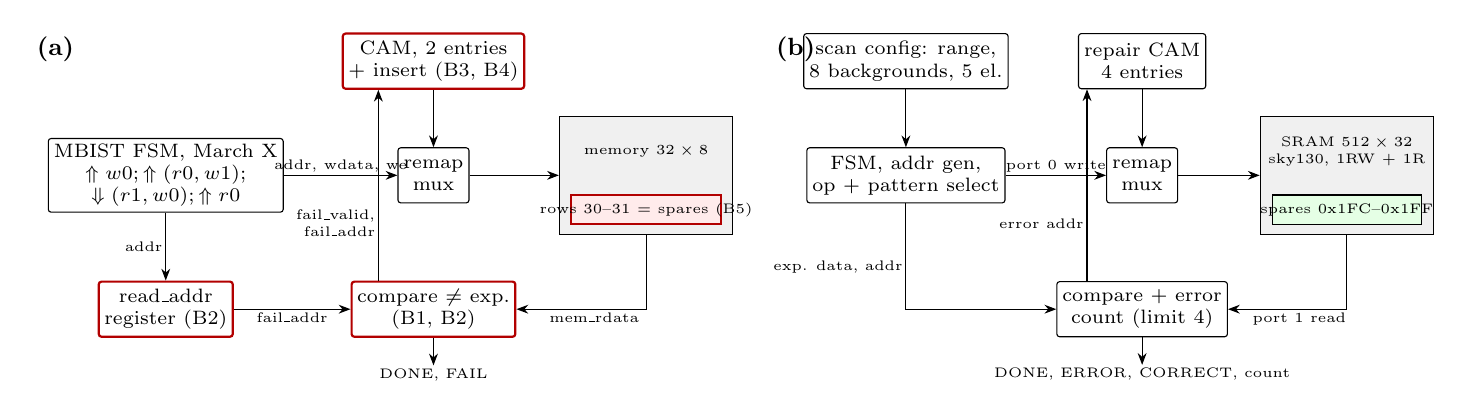
\begin{tikzpicture}[font=\scriptsize, >={Stealth[length=1.5mm]},
  blk/.style={draw, rounded corners=1pt, align=center, inner sep=2pt, minimum height=7mm},
  mem/.style={draw, fill=black!6, align=center, inner sep=2pt, minimum width=22mm, minimum height=15mm},
  bad/.style={draw=red!70!black, thick},
  lab/.style={font=\tiny, inner sep=1pt}]
% ---------------- (a) Design A ----------------
\begin{scope}
\node[font=\small\bfseries] at (-1.4,1.6) {(a)};
\node[blk, minimum width=22mm] (fsmA) at (0,0) {MBIST FSM, March X\\$\Uparrow w0;\Uparrow(r0,w1);$\\$\Downarrow(r1,w0);\Uparrow r0$};
\node[blk] (remA) at (3.4,0) {remap\\mux};
\node[mem] (memA) at (6.1,0) {};
\node[font=\tiny, align=center] at (6.1,0.3) {memory $32\times8$};
\draw[bad, fill=red!8] (5.15,-0.62) rectangle (7.05,-0.25);
\node[font=\tiny] at (6.1,-0.44) {rows 30--31 = spares (B5)};
\node[blk, bad, minimum width=18mm] (cmpA) at (3.4,-1.7) {compare $\ne$ exp.\\(B1, B2)};
\node[blk, bad, minimum width=14mm] (raA) at (0,-1.7) {read\_addr\\register (B2)};
\node[blk, bad] (camA) at (3.4,1.45) {CAM, 2 entries\\+ insert (B3, B4)};
\draw[->] (fsmA.east) -- node[lab, above] {addr, wdata, we} (remA.west);
\draw[->] (remA.east) -- (memA.west);
\draw[->] (memA.south) |- node[lab, pos=0.7, below] {mem\_rdata} (cmpA.east);
\draw[->] (fsmA.south) -- node[lab, left] {addr} (raA.north);
\draw[->] (raA.east) -- node[lab, below] {fail\_addr} (cmpA.west);
\draw[->] ([xshift=-7mm]cmpA.north) -- node[lab, left, pos=0.3, align=right] {fail\_valid,\\fail\_addr} ([xshift=-7mm]camA.south);
\draw[->] (camA.south) -- (remA.north);
\draw[->] (cmpA.south) -- ++(0,-0.35) node[lab, below] {DONE, FAIL};
\end{scope}
% ---------------- (b) Design B ----------------
\begin{scope}[xshift=9.4cm]
\node[font=\small\bfseries] at (-1.4,1.6) {(b)};
\node[blk, minimum width=18mm] (cfgB) at (0,1.45) {scan config: range,\\8 backgrounds, 5 el.};
\node[blk, minimum width=18mm] (fsmB) at (0,0) {FSM, addr gen,\\op + pattern select};
\node[blk] (remB) at (3.0,0) {remap\\mux};
\node[mem] (memB) at (5.6,0) {};
\node[font=\tiny, align=center] at (5.6,0.3) {SRAM $512\times32$\\sky130, 1RW + 1R};
\draw[fill=green!10] (4.65,-0.62) rectangle (6.55,-0.25);
\node[font=\tiny] at (5.6,-0.44) {spares 0x1FC--0x1FF};
\node[blk, minimum width=18mm] (cmpB) at (3.0,-1.7) {compare + error\\count (limit 4)};
\node[blk] (camB) at (3.0,1.45) {repair CAM\\4 entries};
\draw[->] (cfgB) -- (fsmB);
\draw[->] (fsmB.east) -- node[lab, above] {port 0 write} (remB.west);
\draw[->] (remB.east) -- (memB.west);
\draw[->] (memB.south) |- node[lab, pos=0.7, below] {port 1 read} (cmpB.east);
\draw[->] (fsmB.south) |- node[lab, pos=0.3, left] {exp. data, addr} (cmpB.west);
\draw[->] ([xshift=-7mm]cmpB.north) -- node[lab, left, pos=0.3] {error addr} ([xshift=-7mm]camB.south);
\draw[->] (camB.south) -- (remB.north);
\draw[->] (cmpB.south) -- ++(0,-0.35) node[lab, below] {DONE, ERROR, CORRECT, count};
\end{scope}
\end{tikzpicture}
\caption{Architecture of the two designs under test. (a) Design A (TT \#777): red blocks are where bugs B1--B5 of Table~\ref{tab:bugs} sit; the spare rows lie inside the tested range. (b) Design B (mbist\_ctrl): programmable algorithm and data backgrounds, separate write and read ports, spares outside the tested range.}
\label{fig:arch}
\end{figure*}


\section{Designs and Experimental Setup}
\label{sec:setup}
\textbf{Design A} (Fig.~\ref{fig:arch}a) is Tiny Tapeout IHP~26a project \#777 \cite{tt777}, an
MBIST with a CAM-style BISR, at its taped-out commit (Apache-2.0). The RTL implements a
$32\times8$ memory with two repair entries remapped to rows 30--31, which are also ordinary tested
addresses; the documentation describes a $256\times8$ memory with 16 entries. Although documented
as March C--, the controller implements March X,
$\{\Uparrow(w0);\Uparrow(r0,w1);\Downarrow(r1,w0);\Uparrow(r0)\}$.

\textbf{Design B} (Fig.~\ref{fig:arch}b) is mbist\_ctrl \cite{mbistctrl} (Apache-2.0), taped out
on an Efabless/SkyWater shuttle. It tests a $512\times32$ two-port SRAM with a programmable
controller; by default eight data backgrounds $\times$ five March elements with read-after-write
in both directions, over words 0x000--0x1FB, with four spare words 0x1FC--0x1FF and an error limit
of four. We simulate the MBIST core with the SkyWater SRAM behavioural model wired as on the chip,
with standard cells replaced by behavioural equivalents. Its golden model works at the repair
level: for a set $W$ of faulty user words a correct design reports ERROR\,=\,0, CORRECT\,=\,1,
count $|W|$ and repair table $W$ if $|W|\le4$, and ERROR\,=\,1 otherwise.

\textbf{Campaigns} (Table~\ref{tab:setup}). Design~A: SAF0/1 and TF$\uparrow\downarrow$ in all 256
cells and idempotent CFs with physically adjacent aggressors (row above, row below, neighbouring
bit), both transitions and forced values. Design~B: an SAF in every user word, a TF in every
second word, 30 random sets each of 2--6 faulty words and 20 faulty-spare cases. Seeded bugs: 16
in Design~A (controller and BISR) and 18 in Design~B (address generator, comparator, repair,
FSM, pattern and stimulus selection).

\begin{table}[t]
\centering
\caption{Designs and campaign sizes.}
\label{tab:setup}
\setlength{\tabcolsep}{3pt}
\begin{tabular}{@{}lrr@{}}
\toprule
 & Design A (TT \#777) & Design B (mbist\_ctrl) \\
\midrule
Memory / spares        & $32\times8$ / 2 rows & $512\times32$ / 4 words \\
Algorithm              & March X, solid data   & 5 el.\ $\times$ 8 backgrounds \\
Fault runs             & 4{,}032               & 1{,}694 \\
Seeded bugs $\times$ tests & $16\times129$     & $18\times7$ \\
Cycles per MBIST run$^\ast$ & 228            & 162{,}563 \\
Simulation time per run & 0.01\,s             & 2.05\,s \\
\bottomrule
\end{tabular}
\\[2pt]\footnotesize $^\ast$Fault-free run, from start to DONE; Icarus Verilog 14.0 (devel).
\end{table}

\textbf{Tools.} Icarus Verilog 14.0 \cite{icarus}; Python for the golden model, campaigns,
statistics and plots. The directed tests behind Table~\ref{tab:bugs} were also reproduced on the
EDA Playground web service with Icarus Verilog 12.0.

\section{Results}
\label{sec:results}
\subsection{Design A: detection and escapes}
\label{sec:resA}
The golden model predicts that March X detects 2{,}528 of the 4{,}032 faults; the DUT raises FAIL
in 2{,}456 (Table~\ref{tab:summary}, Fig.~\ref{fig:detect}). All 72 differences are escapes, a
faulty memory that passes (2.85\%, 95\% CI 2.27--3.57\%); there are no false fails. Every escape
sits at address 0 or 31 (Fig.~\ref{fig:escmap}), the last address of the $\Downarrow(r1,w0)$
element and of the final $\Uparrow(r0)$ element.

\begin{table}[t]
\centering
\caption{Fault campaign on Design A (single faults).}
\label{tab:summary}
\setlength{\tabcolsep}{3.5pt}
\begin{tabular}{@{}lrrrrr@{}}
\toprule
Class & Faults & Golden det. & DUT FAIL & Escapes & Correct$^\ast$ \\
\midrule
SAF            & 512   & 512   & 504   & 8  & 0 \\
TF             & 512   & 512   & 496   & 16 & 0 \\
CF inter-word  & 1{,}984 & 992 & 960   & 32 & 0 \\
CF intra-word  & 1{,}024 & 512 & 496   & 16 & 0 \\
\midrule
Total          & 4{,}032 & 2{,}528 & 2{,}456 & 72 & 0 \\
\bottomrule
\end{tabular}
\\[2pt]\footnotesize $^\ast$Detected runs whose fail addresses and repair table both match the golden model.
\end{table}

\begin{figure}[t]
\centering
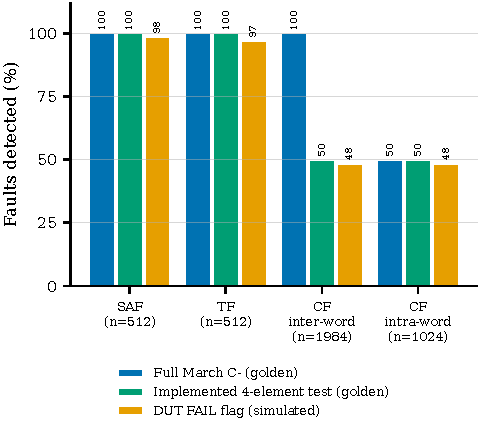
\includegraphics[width=\columnwidth]{fig_detection.pdf}
\caption{Fault detection by class: full March C-- and the implemented March X (golden model) versus Design A's FAIL flag.}
\label{fig:detect}
\end{figure}

\begin{figure}[t]
\centering
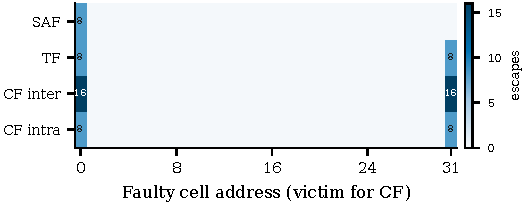
\includegraphics[width=\columnwidth]{fig_escape_map.pdf}
\caption{Design A escapes by faulty-cell address and fault class. All 72 escapes are at addresses 0 and 31, the final addresses of the two descending/final read elements.}
\label{fig:escmap}
\end{figure}

\subsection{What each checker level sees}
Fig.~\ref{fig:checkers} shows, for every detectable fault, whether its run exposes a bug. The
design's own testbench (L0) passes every run. L1 exposes the 72 escapes. L2 exposes a bug in all
2{,}528 detectable faults (95\% CI 99.85--100\%): in every detected run the fail addresses and the
repair table differ from the prediction. Of 2{,}712 fail reports that pair with a predicted report,
only 280 (10.3\%) carry the correct address; 2{,}416 are off by one. The faulty cell reached the
repair table in only 40 of 2{,}456 failing runs (1.63\%, CI 1.20--2.21\%), and in every failing run
both repair entries held the same address.

\begin{figure}[t]
\centering
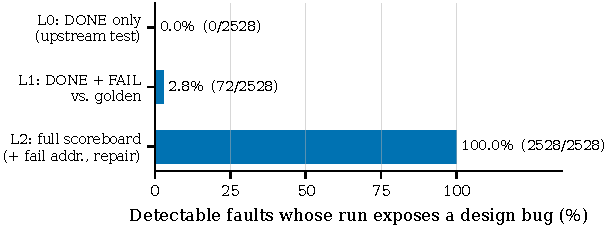
\includegraphics[width=\columnwidth]{fig_checkers.pdf}
\caption{Detectable fault runs that expose a design bug, by checker level, for both designs.}
\label{fig:checkers}
\end{figure}

\subsection{Root causes}
\label{sec:root}
Table~\ref{tab:bugs} lists the bugs, each reproduced in simulation and B1--B3 traced in waveforms.
Fig.~\ref{fig:rootcause} shows the common cause of B1 and B2 at register level: the read data
reaches the comparator two stages after its address, while the fail address comes from a register
that advances one stage earlier. Fig.~\ref{fig:wave} shows B1 on the waveform: the read of
address~0 returns FE, but the element has ended when the data arrives, so FAIL stays low.

\begin{table}[t]
\centering
\caption{Design bugs found in Design A.}
\label{tab:bugs}
\setlength{\tabcolsep}{3pt}
\begin{tabular}{@{}lp{3.4cm}p{3.1cm}@{}}
\toprule
ID & Symptom & Root cause \\
\midrule
B1 & Escapes at addresses 0 and 31 (72 runs) & Last read of $\Downarrow(r1,w0)$ and of final $\Uparrow(r0)$ never compared \\
B2 & Fail address off by one & Compare uses a read-address register that has advanced \\
B3 & One failure fills both repair entries & Non-blocking ``inserted'' flag read in the same cycle \\
B4 & Second faulty cell never recorded & Table already full of duplicates (B3); seen with two injected faults \\
B5 & Spares overlap user space & Spare rows 30--31 are also tested user addresses \\
B6 & Docs vs.\ RTL mismatch & $256\times8$/16 entries documented; $32\times8$/2 implemented \\
\bottomrule
\end{tabular}
\end{table}

% Root cause of B1/B2: read pipeline of Design A at register level -- included by main.tex
\begin{figure}[t]
\centering
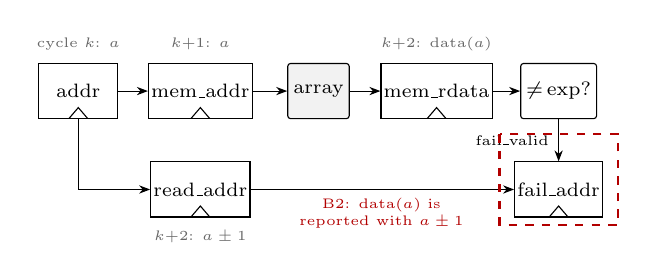
\begin{tikzpicture}[font=\scriptsize, >={Stealth[length=1.4mm]},
  ff/.style={draw, minimum width=10mm, minimum height=7mm, align=center, inner sep=1pt,
             path picture={\draw ([xshift=-1.2mm]path picture bounding box.south) -- ++(1.2mm,1.4mm) -- ++(1.2mm,-1.4mm);}},
  lg/.style={draw, rounded corners=1pt, align=center, inner sep=2pt, minimum height=7mm},
  cyc/.style={font=\tiny, text=black!60}]
\node[ff] (addr) at (0,0) {addr};
\node[ff] (ma)   at (1.55,0) {mem\_addr};
\node[lg, fill=black!5] (arr) at (3.05,0) {array};
\node[ff] (mrd)  at (4.55,0) {mem\_rdata};
\node[lg] (cmp)  at (6.1,0) {$\ne$\,exp?};
\node[ff] (ra)   at (1.55,-1.25) {read\_addr};
\node[ff] (fa)   at (6.1,-1.25) {fail\_addr};
\node[cyc] at (0,0.6) {cycle $k$: $a$};
\node[cyc] at (1.55,0.6) {$k{+}1$: $a$};
\node[cyc] at (4.55,0.6) {$k{+}2$: data($a$)};
\node[cyc] at (1.55,-1.85) {$k{+}2$: $a\pm1$};
\draw[->] (addr) -- (ma);
\draw[->] (ma) -- (arr);
\draw[->] (arr) -- (mrd);
\draw[->] (mrd) -- (cmp);
\draw[->] (cmp) -- node[font=\tiny, left] {fail\_valid} (fa);
\draw[->] (addr.south) |- (ra.west);
\draw[->] (ra.east) -- (fa.west);
\draw[red!70!black, thick, dashed] (5.35,-0.55) rectangle (6.85,-1.7);
\node[font=\tiny, text=red!70!black, align=center] at (3.85,-1.55) {B2: data($a$) is\\reported with $a\pm1$};
\end{tikzpicture}
\caption{Register-level view of Design A's read pipeline (boxes with a clock mark are registers). The read data reaches the comparator two stages after its address, but the fail address is taken from a register that has already advanced (B2). For the same reason the last read of an element is still in flight when the FSM leaves the element, so it is never compared (B1).}
\label{fig:rootcause}
\end{figure}


\begin{figure*}[t]
\centering
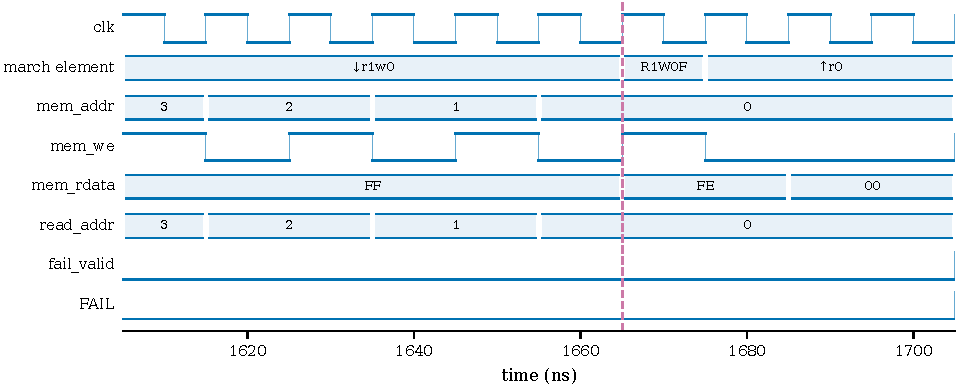
\includegraphics[width=\textwidth]{fig_wave_b1.pdf}
\caption{B1 on Design A: stuck-at-0 at address~0. The faulty read data (FE) arrives after $\Downarrow(r1,w0)$ ends (dashed line) and is never compared; fail\_valid never rises and FAIL stays low.}
\label{fig:wave}
\end{figure*}

\subsection{Design B: a control case}
\label{sec:resB}
Table~\ref{tab:mc} summarises Design~B. Every single SAF and TF was detected, counted and repaired
at the faulty word's address; sets of two to four faulty words were repaired exactly; sets of five
or six were reported as unrepairable. No run exposed a bug at any level: 0 of 1{,}674 non-spare
runs (95\% upper bound 0.23\%). Fig.~\ref{fig:wavemc} shows a repair: the read of word~16 returns
5555\,5554 instead of 5555\,5555, the word enters repair entry~0, and from the next access it is
remapped to spare 0x1FC. A faulty spare that is never used has no effect; when it is used, the
controller detects it, consumes the next entry for the same address, and reports ERROR only when
the four entries run out. Code review found a latent off-by-one in the repair-counter bound
($\le$ instead of $<$ the limit), unreachable because the comparator stops reporting at the limit.

\begin{table}[t]
\centering
\caption{Fault campaign on Design B.}
\label{tab:mc}
\setlength{\tabcolsep}{4pt}
\begin{tabular}{@{}lrrr@{}}
\toprule
Case & Runs & ERROR (golden / DUT) & L2 bugs \\
\midrule
Single SAF (all words)       & 1{,}016 & 0 / 0   & 0 \\
Single TF (every 2nd word)   & 508     & 0 / 0   & 0 \\
2--4 faulty words            & 90      & 0 / 0   & 0 \\
5--6 faulty words            & 60      & 60 / 60 & 0 \\
Faulty spare + 0--4 faults   & 20      & -- / 4  & -- \\
\bottomrule
\end{tabular}
\end{table}

\begin{figure}[t]
\centering
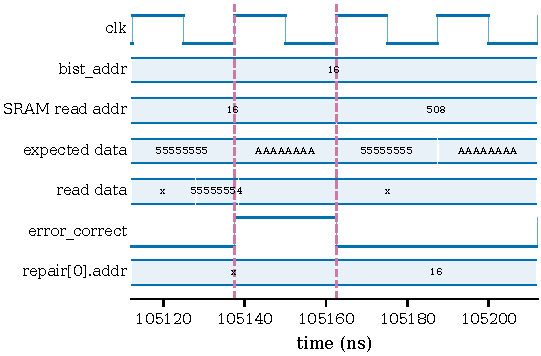
\includegraphics[width=\columnwidth]{fig_wave_mc_repair_narrow.pdf}
\caption{Design B: stuck-at-0 in word 16 is detected (read 55555554, expected 55555555), entered in repair entry 0, and remapped to spare word 0x1FC (508) from the next access.}
\label{fig:wavemc}
\end{figure}

\subsection{Seeded bugs: qualifying the checkers}
\label{sec:mut}
Fig.~\ref{fig:mut} shows the kill rate of the 34 seeded bugs. Completion-only checking kills 5
(15\%; only bugs that change whether or when DONE asserts); the pass/fail flag kills 21 (62\%); the
full scoreboard kills 27 (79\%). On Design~A the step from L1 to L2 adds five bugs (50\% to 81\%),
all in fail-address reporting and repair. On Design~B, CORRECT and the count add one; repair errors
there also change the count, so the repair table adds none. Table~\ref{tab:surv} lists the seven
survivors: four do not change any output (equivalent), and three are masked by the test set, most
notably ``stops after the first data background'', which only intra-word CFs would expose.

\begin{figure}[t]
\centering
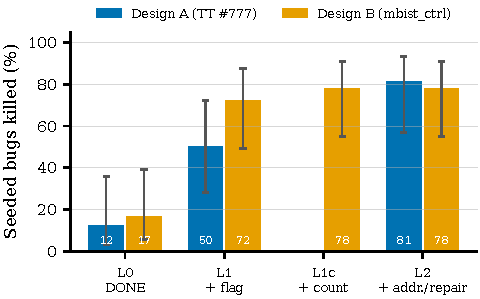
\includegraphics[width=\columnwidth]{fig_mutants.pdf}
\caption{Seeded RTL bugs killed per checker level (error bars: Wilson 95\% CI). L1c applies to Design B only.}
\label{fig:mut}
\end{figure}

\begin{table}[t]
\centering
\caption{Seeded bugs that survive all checker levels.}
\label{tab:surv}
\setlength{\tabcolsep}{3pt}
\begin{tabular}{@{}lp{3.5cm}p{3.1cm}@{}}
\toprule
ID & Seeded change & Why it survives \\
\midrule
A06 & FAIL not set by first r0 element & Masked: same faults also fail later reads \\
A07 & Fail address from \texttt{addr} not \texttt{read\_addr} & Equivalent in this element \\
A14 & Duplicate check disabled & Equivalent given B3 \\
B08 & Comparator CORRECT never set & Top-level CORRECT comes from repair block \\
B13 & Remap also scans unwritten entry & Equivalent \\
B14 & Stops after first background & Masked: needs intra-word CF \\
B15 & No abort on unrepairable error & Same final outputs \\
\bottomrule
\end{tabular}
\end{table}

\subsection{Algorithm adequacy}
Independently of the RTL, the golden model compares algorithms on the same fault list
(Fig.~\ref{fig:alg}). Design~A's March X detects 50\% of inter-word CFs where March C-- detects
100\%; with solid data both detect 50\% of intra-word CFs. Design~B's default algorithm and March
C-- with four backgrounds detect all four classes.

\begin{figure}[t]
\centering
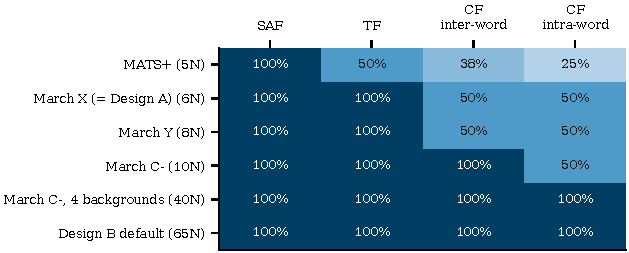
\includegraphics[width=\columnwidth]{fig_algorithms.pdf}
\caption{Golden-model coverage of March algorithms on a $32\times8$ memory (same fault list as Table~\ref{tab:summary}); operations per word in parentheses.}
\label{fig:alg}
\end{figure}

\section{Discussion}
\label{sec:disc}
\subsection{Recommendations for MBIST/BISR Designers}
The bugs suggest rules that are cheap in new designs: (1) carry the address with the read data
through the pipeline and report the address that travelled with the failing data, not a
controller register; (2) drain every outstanding read before leaving a March element or the test;
(3) make repair insertion a one-hot priority write with a same-cycle duplicate check; (4) keep
spare resources outside the tested address space, or test them first; (5) expose the fail-address
stream and repair registers to the testbench, since a pass/fail flag hides most bugs; and (6)
qualify the testbench with seeded bugs, as completion-only checks kill fewer than one in five.

\subsection{Limitations and Open Questions}
The study is simulation-only and uses small open-source memories; industrial MBIST adds
programmable algorithms, shared controllers and physical address scrambling. Faults are
behavioural; for Design~A they are single faults, so multi-fault repair (B4) was examined with
directed tests, while Design~B was run with up to six faulty words. The golden models encode an
interpretation of each design's intent (spares outside the tested range, repair of the first $R$
distinct addresses). Design~B's seeded-bug test set is small (seven tests); adding intra-word CFs
would expose B14. Open questions are a chip-level run with several MBIST instances behind one bus
and formal equivalence between the golden model and the controller's algorithm encoding.

\section{Conclusion}
Checking only completion and the pass/fail flag gives false confidence in MBIST and repair logic.
On a taped-out open-source design, a golden-model scoreboard exposed escapes, wrong fail addresses
and a broken repair table in every detectable fault, none of which the design's own testbench
detected, and raised no false alarm on a second, well-built design. Seeded bugs confirm that each
added checker level kills bugs the weaker ones miss. Designs, testbenches, scripts and results are
available at \url{https://github.com/abhinavkidambi1989/p0-mbist-verif} (public upon publication).

\section*{Acknowledgment}
The author used an AI assistant (Claude, Anthropic) to help draft text, testbench code, scripts
and figures. All content was reviewed, verified and revised by the author, who takes full
responsibility for it.

\begin{thebibliography}{99}
\bibitem{zorian2003} Y.~Zorian and S.~Shoukourian, ``Embedded-memory test and repair: Infrastructure IP for SoC yield,'' \emph{IEEE Design \& Test of Computers}, vol.~20, no.~3, pp.~58--66, 2003.
\bibitem{vandegoor1991} A.~J. van de Goor, \emph{Testing Semiconductor Memories: Theory and Practice}. Chichester, U.K.: Wiley, 1991.
\bibitem{vandegoor1993} A.~J. van de Goor, ``Using March tests to test SRAMs,'' \emph{IEEE Design \& Test of Computers}, vol.~10, no.~1, pp.~8--14, 1993.
\bibitem{knaizuk1977} J.~Knaizuk and C.~R.~P. Hartmann, ``An optimal algorithm for testing stuck-at faults in random access memories,'' \emph{IEEE Trans. Computers}, vol.~C-26, no.~11, pp.~1141--1144, 1977.
\bibitem{marinescu1982} M.~Marinescu, ``Simple and efficient algorithms for functional RAM testing,'' in \emph{Proc. IEEE Int. Test Conf. (ITC)}, 1982, pp.~236--239.
\bibitem{vandegoor1996} A.~J. van de Goor, G.~N. Gaydadjiev, V.~N. Yarmolik, and V.~G. Mikitjuk, ``March LR: A test for realistic linked faults,'' in \emph{Proc. IEEE VLSI Test Symp.}, 1996.
\bibitem{alharbi2003} S.~M. Al-Harbi and S.~K. Gupta, ``Generating complete and optimal March tests for linked faults in memories,'' in \emph{Proc. IEEE VLSI Test Symp.}, 2003.
\bibitem{vandegoor1994} A.~J. van de Goor and B.~Smit, ``Automating the verification of memory tests,'' in \emph{Proc. IEEE VLSI Test Symp.}, 1994, pp.~312--318.
\bibitem{kumar2021} A.~Kumar, ``Assertion based functional verification of March algorithm based MBIST controller,'' arXiv:2106.11461, 2021.
\bibitem{tulsyan2026} S.~Tulsyan, V.~Pillai~A, M.~Jalasutram, P.~Sinha, and M.~Parasrampuria, ``Physical design aware verification methodology for closing coverage gaps in SharedBus MBIST,'' IEEE, 2026, IEEE Xplore doc.~11646504.
\bibitem{sontakke2024} V.~Sontakke and D.~Atchina, ``Memory built-in self-repair and correction for improving yield: A review,'' \emph{Int. J. Electrical and Computer Engineering}, vol.~14, no.~1, pp.~140--156, 2024.
\bibitem{demillo1978} R.~A. DeMillo, R.~J. Lipton, and F.~G. Sayward, ``Hints on test data selection: Help for the practicing programmer,'' \emph{Computer}, vol.~11, no.~4, pp.~34--41, 1978.
\bibitem{jia2011} Y.~Jia and M.~Harman, ``An analysis and survey of the development of mutation testing,'' \emph{IEEE Trans. Software Engineering}, vol.~37, no.~5, pp.~649--678, 2011.
\bibitem{wilson1927} E.~B. Wilson, ``Probable inference, the law of succession, and statistical inference,'' \emph{J. American Statistical Association}, vol.~22, no.~158, pp.~209--212, 1927.
\bibitem{tt777} Tiny Tapeout, ``IHP 26a project \#777: MBIST with MBISR,'' \url{https://tinytapeout.com/chips/ttihp26a/777}, accessed Nov.~13, 2026.
\bibitem{mbistctrl} D.~Annayya, ``mbist\_ctrl,'' \url{https://github.com/dineshannayya/mbist_ctrl}, accessed Nov.~13, 2026.
\bibitem{icarus} S.~Williams, ``Icarus Verilog,'' \url{https://github.com/steveicarus/iverilog}.
\end{thebibliography}

\end{document}
